\documentclass[12pt,]{article}
\usepackage[T1]{fontenc}
\usepackage{lmodern}
\usepackage{amssymb,amsmath}
\usepackage{ifxetex,ifluatex}
\usepackage{fixltx2e} % provides \textsubscript
% use upquote if available, for straight quotes in verbatim environments
\IfFileExists{upquote.sty}{\usepackage{upquote}}{}
\ifnum 0\ifxetex 1\fi\ifluatex 1\fi=0 % if pdftex
  \usepackage[utf8]{inputenc}
\else % if luatex or xelatex
  \ifxetex
    \usepackage{mathspec}
    \usepackage{xltxtra,xunicode}
  \else
    \usepackage{fontspec}
  \fi
  \defaultfontfeatures{Mapping=tex-text,Scale=MatchLowercase}
  \newcommand{\euro}{€}
\fi
% use microtype if available
\IfFileExists{microtype.sty}{\usepackage{microtype}}{}
\usepackage[margin=1in]{geometry}
\usepackage{graphicx}
% Redefine \includegraphics so that, unless explicit options are
% given, the image width will not exceed the width of the page.
% Images get their normal width if they fit onto the page, but
% are scaled down if they would overflow the margins.
\makeatletter
\def\ScaleIfNeeded{%
  \ifdim\Gin@nat@width>\linewidth
    \linewidth
  \else
    \Gin@nat@width
  \fi
}
\makeatother
\let\Oldincludegraphics\includegraphics
{%
 \catcode`\@=11\relax%
 \gdef\includegraphics{\@ifnextchar[{\Oldincludegraphics}{\Oldincludegraphics[width=\ScaleIfNeeded]}}%
}%
\ifxetex
  \usepackage[setpagesize=false, % page size defined by xetex
              unicode=false, % unicode breaks when used with xetex
              xetex]{hyperref}
\else
  \usepackage[unicode=true]{hyperref}
\fi
\hypersetup{breaklinks=true,
            bookmarks=true,
            pdfauthor={},
            pdftitle={},
            colorlinks=true,
            citecolor=blue,
            urlcolor=blue,
            linkcolor=magenta,
            pdfborder={0 0 0}}
\urlstyle{same}  % don't use monospace font for urls
\setlength{\parindent}{0pt}
\setlength{\parskip}{6pt plus 2pt minus 1pt}
\setlength{\emergencystretch}{3em}  % prevent overfull lines
\setcounter{secnumdepth}{0}

\author{}
\date{}
\usepackage{lineno}
\linenumbers
\usepackage{setspace}
\doublespacing

\begin{document}

\normalsize


\section{How coexistence mechanisms mediate temporal
stability}\label{how-coexistence-mechanisms-mediate-temporal-stability}

\subsubsection{Andrew T. Tredennick, Peter B. Adler, and Frederick R.
Adler}\label{andrew-t.-tredennick-peter-b.-adler-and-frederick-r.-adler}

\emph{Andrew T. Tredennick
(\href{mailto:atredenn@gmail.com}{\href{mailto:atredenn@gmail.com}{atredenn@gmail.com}}),
Department of Wildland Resources and the Ecology Center, Utah State
University, Logan, UT}

\emph{Peter B. Adler, Department of Wildland Resources and the Ecology
Center, Utah State University, Logan, UT}

\emph{Frederick R. Adler, Departments of Biology and Mathematics,
University of Utah, Salt Lake City, UT}

\subsection{Introduction}\label{introduction}

Theoretical work aimed toward identifying the mechanisms by which
species richness promotes temporal stability has treated species
coexistence as a foregone conclusion. In so doing, that large body of
work implicitly assumes that the interaction between environmental
variability and the mechanism(s) by which species coexist is trivial.
However, under the same conditions of environmental variability,
population dynamics will respond differently depending on the
coexistence context. In turn, this leads to different dynamics at the
community and ecosystem levels depending on how species interact. So, it
stands to reason that identifying the key mechanisms that promote
ecosystem stability requires a solid understanding of how species
coexistence mediates temporal stability in fluctuating environments.

To that end, we will analyze a general consumer-resource model under
different coexistence assmptions. Our starting point is a model of two
plant consumers and one resource (e.g., soil moisture or nitrogen). We
will focus on three cases of species coexistence:

\begin{enumerate}
  \item Relative nonlinearty
  \item Temporal storage effect
  \item A combination of both mechanisms
\end{enumerate}

Each scenario requires different model assumptions and structure, so we
will describe each in turn. Although the structure may change slightly
to incorporate different coexistence mechanisms, the strength of our
approach lies in the similarities among the models since we work under a
unified consumer-resource framework.

\subsubsection{A general consumer-resource
model}\label{a-general-consumer-resource-model}

\begin{figure}[htbp]
\centering
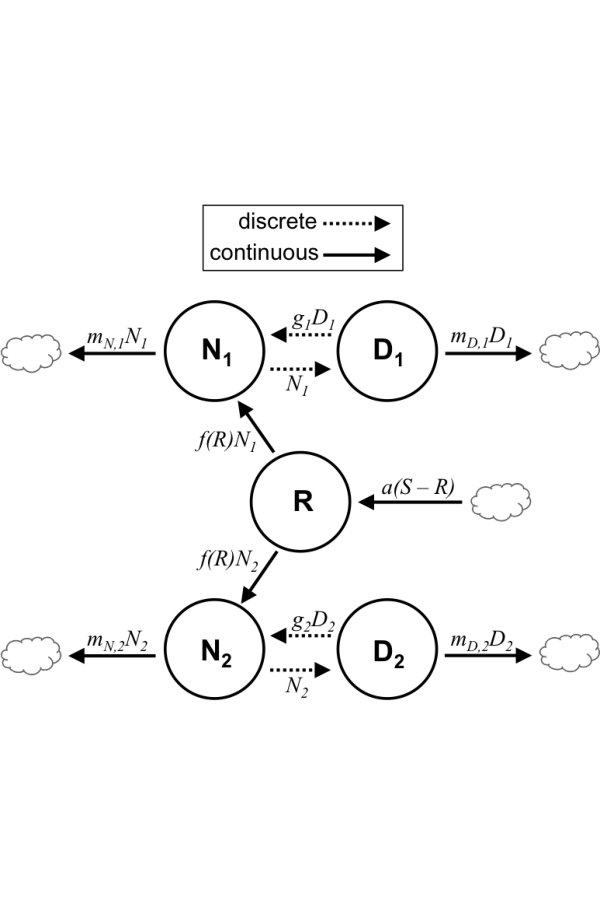
\includegraphics{components/figure/manuscript-figure_1.pdf}
\caption{Diagram of our semi-discrete consumer-resource model. Solid
lines show continuous dynamics while dashed lines show the discrete
transitions.}
\end{figure}

We start with a general consumer-resource model where the consumer can
be in one of two-states: a dormant state $D$ and a live state $N$
(Figure\textasciitilde{}\ref{fig:model}). Transitions between $N$ and
$D$ occur at discrete intervals $T$, so our model is formulated as
``pulsed differential equations``. For clarity we refer to $T$ as years
and the growing time between years, $\tau$, as seasons. Seasonal
(within-year) dynamics are modeled as three differential equations:

\begin{align}
\frac{\text{d}D_{i}}{\text{d}\tau} &= -(m_{D,i}D_{i})\\
\frac{\text{d}N_{i}}{\text{d}\tau} &= f(R)N_{i} - m_{N,i}N_{i}\\
\frac{\text{d}R_{i}}{\text{d}\tau} &= a(S - R) - \sum\limits_{i=1,2}f(R)N_{i}
\end{align}

where $i$ denotes species, $D$ is the dormant (long-lived) biomass
state, $N$ is the living biomass (fast-growing, shorter-lived) state,
and $m$s are biomass loss rates. The growth rate of living biomass is a
resource-dependent function, $f(R) = r_{i}R/(K_{i}+R)$, where $r$ is the
maximum growth rate and $K$ is the resource level at which growth is
one-half $r$. For the resource dynamics, whose state is denoted by $R$,
we use a linear resource renewal equation where $a$ scales resource
turnover rate and $S$ is the resource equilibrium when consumers are
absent, and an offtake of the resource equal to the sum of each species'
consumption, $\sum_{i=1,2}f(R)N_{i}$. Note that since transitions
between $N$ and $D$ are pulsed, only biomass loss occurs throughout the
season for $D$.

At the beginning of each season we start with initial conditions defined
as $V_{t}$, $W_{t}$, and $Z_{t}$ for the dormant state, the live state,
and the resource, respectively. So for each season, Eqs. 1-3 are solved
given the initial conditions:

\begin{align}
  D_{i}(0) &= V_{i,t} \\
  N_{i}(0) &= W_{i,t} \\
  R(0) &= Z_{t}
\end{align}

The consumers transition between $N$ and $D$ instantaneously between
years. We assume resource density does not change between years. So, at
the yearly transition:

\begin{align}
  V_{i,t+1} &= [N_{i}(T^-)+D_{i}(T^-)](1-g_{t}) \\
  W_{i,t+1} &= [N_{i}(T^-)+D_{i}(T^-)]g_{t} \\
  Z_{t+1} &= R(T^-)
\end{align}

where $D(T^-)$, $N(T^-)$, and $R(T^-)$ are the densities of each state
at the end of the year and $g$ is a time-fluctuating activation rate
that regulates how much dormant biomass is converted to growing-season
live biomass each year. Our formulation assumes that at the end of each
season all accumulated living biomass {[}$N(T^-)${]} is converted to
dormant biomass.

\begin{center}
\begin{table}
\caption{Definition of model parameters.}
\begin{tabular}{l l}
\hline
Parameter & Definition \\
\hline
$m_{D}$ & dormant state mortality rate \\
$r$ & live state maximum resource uptake rate \\
$K$ & live state half-saturation constant for resource uptake rate \\
$m_{N}$ & live state mortality rate \\
$a$ & resource turnover rate \\
$S$ & resource supply rate \\
$g$ & dormant-to-live biomass transition fraction \\ 
\hline
\end{tabular}
\end{table}
\end{center}

\subsubsection{Implementing the storage
effect}\label{implementing-the-storage-effect}

To make this a ``storage-effect" model, we need to satisfy three
conditions: (1) the organisms must have a mechanism for persistence
under unfavorable conditions, (2) species must respond differently to
environmental conditions, and (3) the effects of competition on a
species must be more strongly negative in good years relative to
unfavorable years. Our model meets condition 1 because we include a
dormant stage with very low death rates. We satisfy condition 2 with our
model whenever $g$ is not perfectly correlated between species. Lastly,
our model meets condition 3 because condition 2 partitions intraspecific
and interspecific competition into different years. Thus, during a high
$g$ year for one species, resource uptake is also inherently high for
that species, which increases intraspecific competition relative to
interspecific competition. So, given adequate variability in $g$, the
inferior competitor (species with lower $r$) can persist.

Following Adler and Drake (2008), we generated sequences of
(un)correlated dormant-to-live state transition rates ($g$) for each
species by drawing from multivariate normal distributions with mean 0
and a variance-covariance matrix of

\begin{align}
\begin{bmatrix}
\sigma^2_{E} & \rho\sigma^2_{E} \\
\rho\sigma^2_{E} & \sigma^2_{E}
\end{bmatrix}
\end{align}

\noindent{}where $\sigma^2_{E}$ is the variance and $\rho$ is the
correlation between between the two species' transition rates. For
environmental variability, here induced as variability in $g$, to
promote coexistence via the storage effect, $\rho$ must be less than 1.
The inferior competitor has the strongest potential to persist when
$\rho=-1$ (perfectly uncorrelated transition rates).

\subsubsection{Implementing relative
nonlinearity}\label{implementing-relative-nonlinearity}

When considering consumer-resource dynamics, species coexistence by
relative nonlinearity requires that each species has different nonlinear
responses to resource availability, and resource availability must
fluctuate through time. In a constant resource environment, the species
with the lowest R* will always exclude the other species. So we can
compare this model to the storage effect model, we still allow the
germination rate \emph{g} to vary, but both species are perfectly
correlate -- that is, $\rho=1$.

\subsection{Results}\label{results}

\subsubsection{Storage effect model}\label{storage-effect-model}

Some preliminary results from running simulations of the storage effect
version of the model at different levels of environmental cue
variability ($\sigma_{E}$) and resource supply variability
($\sigma_{S}$). I ran 20 simulations at each combination of $\sigma_{E}$
and $\sigma_{S}$ shown in Figure\textasciitilde{}\ref{fig:storeEffSims}
(the points are the means across the 20 simulations, each run for 2,000
time-steps, with the initial 1,000 time-steps discarded before
calculating anything). There is a weak trend of community CV to saturate
at high levels of resource supply variability
(Figure\textasciitilde{}\ref{fig:storeEffSims}, top panel).

One of the things we are interested in is how well the community buffers
itself against resource variability. Really I should calculate some kind
of asynchrony metric, but for now I just looked at the ratio of the
resource CV to the community CV
(Figure\textasciitilde{}\ref{fig:storeEffSims}, bottom panel). Kind of
difficult to interpret, but it is interesting that at high levels of
variability in the environmental cue that drives the storage effect, the
ratio decreases with resource supply variability. The opposite occurs at
lower levels of variability in the environmental cue.

\pagebreak{}

\subsection{References}\label{references}

Adler, P. B., and J. M. Drake. 2008. Environmental variation, stochastic
extinction, and competitive coexistence. The American naturalist
172:186--195.

\end{document}
